In this \hb{course}, much of the learning will be done by using simulated data, so let's start by learning how to generate data. The basic function to generate random data is \code{runif()} which is used to draw random numbers, uniformly between 0 and 1. In the following example we create 10,000 random draws from a uniform distribution, keep these numbers in a variable called simData, and plot a histogram to show the distribution of the data we have generated. The \code{set.seed()} function is used to ensure that every time we run this code, we will get the same set of random numbers. This is called \textit{reproducible code}. 
\begin{knitrout}
\definecolor{shadecolor}{rgb}{0.969, 0.969, 0.969}\color{fgcolor}\begin{kframe}
\begin{alltt}
\hlcom{# Generate 10,000 points from a uniform distribution}
\hlkwd{set.seed}\hlstd{(}\hlnum{210313}\hlstd{)}
\hlstd{n} \hlkwb{<-} \hlnum{10000}
\hlstd{simData} \hlkwb{<-} \hlkwd{runif}\hlstd{(n)}
\hlkwd{hist}\hlstd{(simData)}
\end{alltt}
\end{kframe}\begin{figure}

{\centering 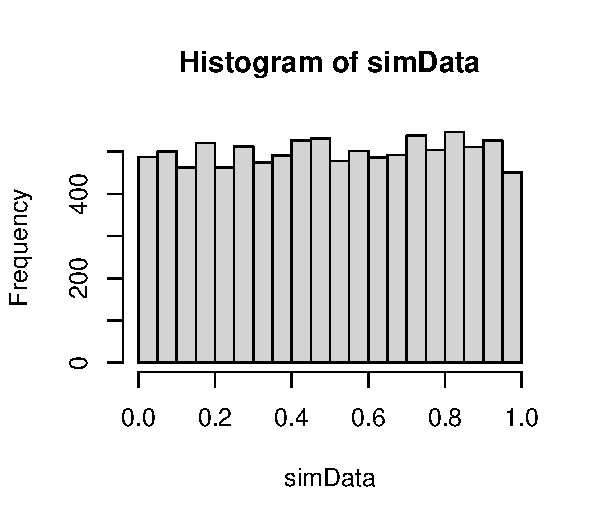
\includegraphics[width=\maxwidth]{figure/intro-runif-1} 

}

\caption[A histogram of 10,000 randomly drawn numbers from a standard uniform distribution]{A histogram of 10,000 randomly drawn numbers from a standard uniform distribution.}\label{fig:intro-runif}
\end{figure}

\end{knitrout}


From the range and the flatness of the histogram we can see that the generated data is indeed uniform on [0,1]. The \code{runif()} function can be used to draw random numbers uniformly on any finite interval. For example, if we want our random numbers to be in the interval [1,5] we will run the following code:

\begin{knitrout}
\definecolor{shadecolor}{rgb}{0.969, 0.969, 0.969}\color{fgcolor}\begin{kframe}
\begin{alltt}
\hlstd{n} \hlkwb{<-} \hlnum{10000}
\hlstd{simData} \hlkwb{<-} \hlkwd{runif}\hlstd{(n,} \hlkwc{min}\hlstd{=}\hlnum{1}\hlstd{,} \hlkwc{max}\hlstd{=}\hlnum{5}\hlstd{)}
\end{alltt}
\end{kframe}
\end{knitrout}

Try it, and draw the histogram as in the previous example. Try it with a fixed seed and verify that you get the same output each time. Then, run the code without a fixed seed and observe that you get a different distribution each time. Since the number of random draws is fairly large, the shape of the histogram will not change much.

From a random draw of a uniform distribution we can generate random numbers from other distributions. For example, we want to simulate (fair) coin flips, and count the number of Heads that we get. Let's say we want to simulate 200 coin tosses. We will draw 200 random numbers from a uniform distribution, and decide that we got Heads in the $i$-th toss if the $i$-the random number is less than 0.5, and Tails otherwise.
Try the following code multiple times (do not use \code{set.seed()}). What do you observe? We will discuss it further in a different \hb{lecture}.
\begin{knitrout}
\definecolor{shadecolor}{rgb}{0.969, 0.969, 0.969}\color{fgcolor}\begin{kframe}
\begin{alltt}
\hlcom{# Simulate 200 coin-flips, using the runif function:}
\hlstd{n.trials} \hlkwb{<-} \hlnum{200}
\hlkwd{cat}\hlstd{(}\hlstr{"Number of Heads is: "}\hlstd{,} \hlkwd{sum}\hlstd{(}\hlkwd{runif}\hlstd{(n.trials)} \hlopt{<} \hlnum{0.5}\hlstd{),} \hlstr{"\textbackslash{}n"}\hlstd{)}
\end{alltt}
\begin{verbatim}
Outout: Number of Heads is:  92
\end{verbatim}
\end{kframe}
\end{knitrout}


A few comments:
\begin{itemize}
\item A comment in \R starts with \#. Any text following the \# sign is considered user-documentation and is not executed by \R.
\item We have used the \code{cat()} function to print (concatenate) text to the console. Fixed text appears in double (or single) quotes, but the content of variables or output from \R functions should not be quoted. The \verb|\n| symbol tells \R to print a newline character at the end. Try to see what happens if you remove it.
\item The expression within the \code{sum()} function produces TRUE/FALSE (Boolean) values. First, we draw n.trials random numbers from a uniform distribution. Then, each one is compared with 0.5. If the value is less than 0.5, the returned value is TRUE. Otherwise, it's FALSE. This demonstrates one of \R's greatest features - allowing to run `vectorized' code. In one line, we generated 200 random numbers and compared each one to 0.5, and as a result, we got 200 Boolean values which we have added together (TRUE counts as 1, and FALSE counts as 0.) So, the result in the sum is the number of Heads in 200 tosses.
\end{itemize}

Statistical inference is based on a mental exercise in which we ask, if we could repeat the same experiment infinitely many times, what would we see? With simulations, we can get a good approximation. For example, the 200 coin-tosses experiment can be repeated, say, 100 times. One way is to use loops, like in the following example:
\begin{knitrout}
\definecolor{shadecolor}{rgb}{0.969, 0.969, 0.969}\color{fgcolor}\begin{kframe}
\begin{alltt}
\hlkwd{set.seed}\hlstd{(}\hlnum{442886}\hlstd{)}
\hlstd{n.trials} \hlkwb{<-} \hlnum{200}  \hlcom{# the number of coin-tosses in each experiment}
\hlstd{reps} \hlkwb{<-} \hlnum{100}  \hlcom{# the number of experiments}
\hlstd{Heads} \hlkwb{<-} \hlkwd{rep}\hlstd{(}\hlnum{0}\hlstd{, reps)}  \hlcom{# A vector to store the results (initialize with 0s)}
\hlkwa{for} \hlstd{(i} \hlkwa{in} \hlnum{1}\hlopt{:}\hlstd{reps) \{}
  \hlstd{Heads[i]} \hlkwb{<-} \hlkwd{sum}\hlstd{((}\hlkwd{runif}\hlstd{(n.trials)} \hlopt{<} \hlnum{0.5}\hlstd{))}
\hlstd{\}}
\hlkwd{hist}\hlstd{(Heads,} \hlkwc{breaks}\hlstd{=}\hlnum{20}\hlstd{)}
\end{alltt}
\end{kframe}\begin{figure}

{\centering 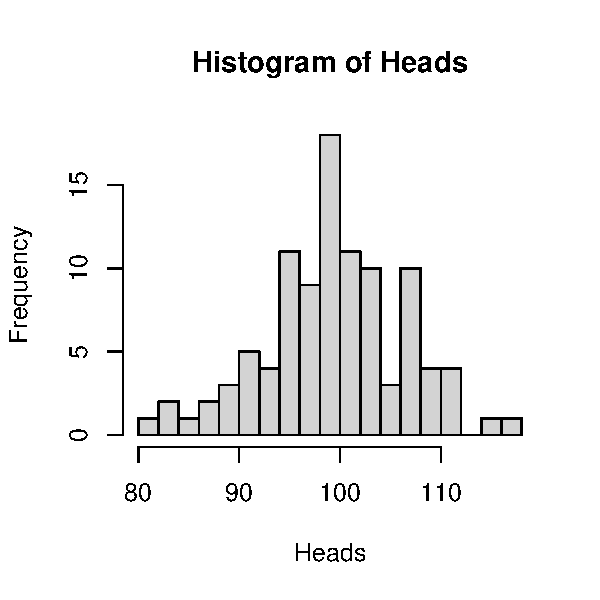
\includegraphics[width=\maxwidth]{figure/intro-heads2-1} 

}

\caption[A histogram of 100 experiments, from each we get the total number of Heads in 200 fair coin tosses]{A histogram of 100 experiments, from each we get the total number of Heads in 200 fair coin tosses.}\label{fig:intro-heads2}
\end{figure}

\end{knitrout}


We've used a \code{for()} loop, with an index variable called \texttt{i} which runs from 1 to 100. In each iteration we simulated n.trials=200 coin tosses, as before. The result from each iteration is stored in the $i$-th position in the vector we called Heads.

Using the uniform distribution, we have created a random draw from a different distribution, called the `binomial'. The mathematical notation is $Bin(N, p)$ where $N$ is the number of trials such that in each trial there can be exactly two outcomes (e.g., coin tosses), and $p$ is the probability of the first possible outcome (e.g., Head), and $1-p$ is the probability of the second possible outcome (e.g., Tail).
\R has a built-in function to generate random numbers from many different distributions, so the code above can be replaced by the following, which uses the \code{rbinom()} function:
\begin{knitrout}
\definecolor{shadecolor}{rgb}{0.969, 0.969, 0.969}\color{fgcolor}\begin{kframe}
\begin{alltt}
\hlkwd{set.seed}\hlstd{(}\hlnum{442886}\hlstd{)}
\hlstd{reps} \hlkwb{<-} \hlnum{100}
\hlstd{n.trials} \hlkwb{<-} \hlnum{200}
\hlstd{Heads} \hlkwb{<-} \hlkwd{rbinom}\hlstd{(reps, n.trials,} \hlnum{0.5}\hlstd{)}
\hlkwd{hist}\hlstd{(Heads,} \hlkwc{breaks}\hlstd{=}\hlnum{20}\hlstd{)}
\end{alltt}
\end{kframe}\begin{figure}

{\centering 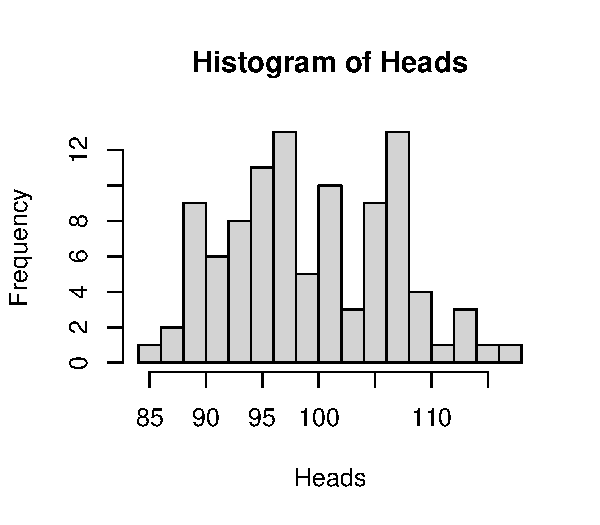
\includegraphics[width=\maxwidth]{figure/intro-binomial-1} 

}

\caption[A histogram of 100 binomial experiments, using rbinom() to simulate 200 fair coin tosses in each experiment]{A histogram of 100 binomial experiments, using rbinom() to simulate 200 fair coin tosses in each experiment.}\label{fig:intro-binomial}
\end{figure}

\end{knitrout}


Exercises:
\begin{enumerate}
\item Change the number of simulated coin-toss datasets (\texttt{reps}) to 1,000 and rerun the code. Then change it to 10,000 and run it again. What do you notice?
\item Change the probability of Heads to 0.2 and run the code again. Then, change it to 0.8. What do you observe?
\item Try other values of the number of trials and the probability of Heads.
\end{enumerate}

